\documentclass[11pt]{article}
\usepackage{graphicx}
\usepackage{amssymb}
%\usepackage[nomarkers]{endfloat}
\usepackage{natbib}
\usepackage{setspace}
\usepackage{wasysym}
\usepackage{wrapfig}
\pagestyle{empty}
\textwidth = 7 in
\textheight = 9 in
\oddsidemargin = -0.5 in
\evensidemargin = -0.5 in
\topmargin = 0.0 in
\headheight = 0.0 in
\headsep = 0.0 in
\parskip = 0.1in
\parindent = 0in
\renewcommand{\Pr}{\mathbb{P}}
\usepackage{paralist}
\usepackage{url}
\newcommand{\href}[2]{\url{#2}}
\usepackage{tikz}
  \usetikzlibrary{shapes.geometric}
  \usetikzlibrary{arrows.meta,arrows}
  \usetikzlibrary{positioning,automata}
\tikzstyle{line}=[draw]
\usepackage{hyperref}
\hypersetup{backref,   linkcolor=blue, citecolor=red, colorlinks=true, hyperindex=true}
\begin{document}
\resizebox{\textwidth}{!}{
    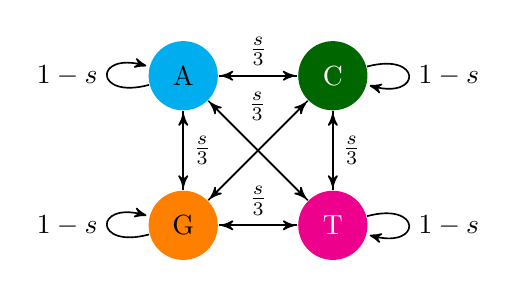
\begin{tikzpicture}[->,>=stealth',shorten >=1pt,auto,semithick,every state/.style={fill=red,draw=none,text=black,shape=ellipse}]
\node[state, fill=cyan] (A) {A};
\node[state, fill=black!60!green,text=white] (C) [right=of A] {C};
\node[state, fill=magenta,text=white] (T) [below=of C] {T};
\node[state, fill=orange,text=black] (G) [below=of A] {G};
\path (A) edge node {$\frac{s}{3}$} (C) ;
\path (A) edge node {$\frac{s}{3}$} (G) ;
\path (A) edge node [pos=.3] {$\frac{s}{3}$} (T) ;
\path (A) edge [loop left] node {$1-s$} (A) ;
\path (C) edge node {} (A) ;
\path (C) edge node {} (G) ;
\path (C) edge node {$\frac{s}{3}$} (T) ;
\path (C) edge [loop right] node {$1-s$} (C) ;
\path (G) edge node {} (A) ;
\path (G) edge node {} (C) ;
\path (G) edge node {$\frac{s}{3}$} (T) ;
\path (G) edge [loop left] node {$1-s$} (G) ;
\path (T) edge node {} (A) ;
\path (T) edge node {} (G) ;
\path (T) edge node {} (C) ;
\path (T) edge [loop right] node {$1-s$} (T) ;
\end{tikzpicture}

}

\end{document}